\documentclass{beamer}
\usepackage{alltt}
\usepackage{tikz}
\usetikzlibrary{matrix}
\usetikzlibrary{trees}
\usepackage{cancel}
\usepackage{subcaption}
\PassOptionsToPackage{obeyspaces}{url}
\usepackage{hyperref}
\usepackage{adjustbox}

\usetheme{Hannover}

\definecolor{darkgreen}{rgb}{0.0, 0.5, 0.0}

\newcommand{\quot}{\texttt{\textquotesingle{}}}
\newcommand{\dquot}{\texttt{"}}
\newcommand{\qquot}{\texttt{\textasciigrave{}}}
\newcommand{\logand}{\texttt{\(\wedge\)}}
\newcommand{\logor}{\texttt{\(\vee\)}}
\newcommand{\sig}{\texttt{\(\Sigma\)}}
\newcommand{\api}{\texttt{API}}
\newcommand{\arrow}{\(\rightarrow\)}
\newcommand{\dotss}{\(\ldots\)}
\newcommand{\vdotss}{\(\vdots\)}
\newcommand{\elist}{\texttt{\textquotesingle{()}}}
\newcommand{\drracket}{\texttt{DrRacket}}
\newcommand{\racket}{\texttt{Racket}}
\newcommand{\nth}{\texttt{n$^{\texttt{th}}$}}
\newcommand{\fsm}{\texttt{FSM}}
\newcommand{\true}{\texttt{\#true}}
\newcommand{\false}{\texttt{\#false}}
\newcommand{\twopartdef}[4]
{
	\left\{
		\begin{array}{ll}
			#1 & \mbox{if } #2 \\
			#3 & \mbox{if } #4
		\end{array}
	\right.
}

\begin{document}

\title{Part I: Fundamental Concepts}
%\subtitle{Using Beamer}
\author{Marco T. Moraz\'{a}n}
\institute{Seton Hall University}
\date{}

\begin{frame}
\titlepage
\end{frame}

\begin{frame}
\frametitle{Outline}
\tableofcontents
\end{frame}

\section{Fundamental Concepts}

\begin{frame}[fragile]
\frametitle{Introduction to \fsm{}}
%\framesubtitle{HOMEWORK}
\begin{scriptsize}
\begin{itemize}
\item<1-> Historically, formal languages and automata theory courses have been theoretical pencil-and-paper courses

\item<1-> Students design algorithms in theory (i.e., without implementing them)

\item<2-> If there is a bug in the algorithm then there is a bug in the proof of a theorem.

\item<3-> Therefore, we focus on implementation.

\item<3-> Unit testing and runtime bugs give you immediate feedback on your implementation providing the opportunity to make corrections before submitting work for grading.

\item<4-> We use a domain specific language called \fsm \ (\textbf{F}unctional \textbf{S}tate \textbf{M}achines)

\item<4-> \fsm \ provides readers of this textbook with the ability to design, program, test, and debug algorithms before writing theorems or submitting for grading

\item<4-> \fsm{} is embedded in \racket{}

\end{itemize}
\end{scriptsize}
\end{frame}

\begin{frame}[fragile]
\frametitle{Introduction to \fsm{}}
%\framesubtitle{HOMEWORK}
\begin{scriptsize}
\begin{itemize}
\item<1-> To write \fsm{} programs the first line in every program must be:
\begin{alltt}
     #lang fsm
\end{alltt}
\item<1-> This line informs \drracket{} that the programming language used is \fsm{}

\item<1-> Provides the testing facilities from \texttt{rackunit}

\item<2-> You may use anything in \racket

\item<3-> A program is never considered complete without unit tests

\item<3-> For the purposes of this textbook, the required syntax is:
\begin{alltt}
     (check-equal? <expression> <expression>)
\end{alltt}

\item<4-> Consider, for example, running the following program:
\begin{alltt}
     #lang fsm

     (check-equal? (= 6 6) #t)
     (check-equal? (* (+ 2 3) (/ 20 2)) 50)
     (check-equal? (string-length "FSM") 4)
\end{alltt}
The result in the interactions window is:
\begin{center}
\includegraphics{error.png}
\end{center}

\end{itemize}
\end{scriptsize}
\end{frame}

\begin{frame}[fragile]
\frametitle{Introduction to \fsm{}}
%\framesubtitle{HOMEWORK}
\begin{scriptsize}
\begin{itemize}
\item<1-> The Design Recipe
\begin{enumerate}
 \item Outline the representation of values.
 \item Outline the computation.
 \item Write the function's signature and purpose.
 \item Write the function's header.
 \item Write unit tests.
 \item Write the function's body.
 \item Run the tests and, if necessary, redesign.
\end{enumerate}

\item<2-> Scaling a binary tree of numbers

\item<3->
\begin{alltt}
;; A binary tree of numbers, (btof number), is either:
;;  1. \elist  2. number  3. (list number (btof number) (btof number))
\end{alltt}

\item<4->
\begin{alltt}
;;; (btof number) \dotss \arrow \dotss
;;; Purpose: \dotss
;(define (f-on-bt a-bt \dotss)
;  (cond [(empty? a-bt)  \dotss]
;        [(number? a-bt) \dotss(f-on-number a-bt)\dotss]
;        [else \dotss(f-on-number (first a-bt))\dotss
;              \dotss(f-on-bt (second a-bt))\dotss
;              \dotss(f-on-bt (third a-bt))\dotss]))
;;; Tests
;(check-equals? (f-on-bt empty \dotss) \dotss)
;(check-equals? (f-on-bt number \dotss) \dotss)
;(check-equals? (f-on-bt (list number \dotss \dotss) \dotss) \dotss)
          \vdotss
\end{alltt}

\end{itemize}
\end{scriptsize}
\end{frame}

\begin{frame}[fragile]
\frametitle{Introduction to \fsm{}}
%\framesubtitle{HOMEWORK}
\begin{scriptsize}
\begin{itemize}
\item<1-> Reason about each subtype independently

\item<2-> If the given binary tree is empty then there is nothing to scale and the resulting tree is empty

\item<3-> If the given binary tree is a leaf then multiply it by the given scalar

\item<4-> If the given binary tree is an interior then make a list with the result of calling \texttt{*} with the root value and the given scalar, making a recursive call with the left subtree and the scalar, and making a recursive call with the right subtree and the scalar

\end{itemize}
\end{scriptsize}
\end{frame}

\begin{frame}[fragile]
\frametitle{Introduction to \fsm{}}
%\framesubtitle{HOMEWORK}
\begin{scriptsize}
\begin{itemize}
\item<1->
\begin{alltt}
     #lang fsm

     ;; (btof number) number \arrow (btof number)
     ;; Purpose: Scale the given (btof number) by the
     ;;          given scalar
     (define (scale-bt a-bt k)
\end{alltt}

\item<3->
\begin{alltt}
     (cond [(empty? a-bt)  a-bt]
           [(number? a-bt) (* k a-bt)]
           [else (list (* k (first a-bt))
                       (scale-bt (second a-bt) k)
                       (scale-bt (third a-bt) k))])
\end{alltt}

\item<2->
\begin{alltt}
     ;; Tests
     ;; empty bt tests
     (check-equal? (scale-bt \elist 10) \elist)
     ;; leaf bt tests
     (check-equal? (scale-bt -50 2) -100)
     (check-equal? (scale-bt 40  8) 320)
     ;; interior node bt tests
     (check-equal? (scale-bt (list 10 \elist (list -8 -4 \elist)) -2)
                   (list -20 \elist (list 16 8 \elist)))
     (check-equal? (scale-bt (list 0
                                   (list 1 2 3)
                                   (list 4
                                         (list 5 \elist \elist)
                                         (list 6 7 8)))
                             3)
                   (list 0
                         (list 3 6 9)
                         (list 12
                               (list 15 \elist \elist)
                               (list 18 21 24))))
\end{alltt}

\end{itemize}
\end{scriptsize}
\end{frame}

\begin{frame}[fragile]
\frametitle{Introduction to \fsm{}}
\framesubtitle{HOMEWORK}
\begin{scriptsize}
\begin{itemize}
\item<1-> Problems: 1--10

\end{itemize}
\end{scriptsize}
\end{frame}

\begin{frame}[fragile]
\frametitle{Introduction to \fsm{}}
%\framesubtitle{HOMEWORK}
\begin{scriptsize}
\begin{itemize}
\item<1-> Two constants that are useful to know before writing \fsm \ programs:
\begin{description}
  \item[\texttt{BLANK}] Denotes a blank space in an input tape.
  \item[\texttt{EMP}] Denotes the empty word (i.e., a word of length 0)
\end{description}

\item<2->
The following are some important \fsm \ data definitions:
\begin{description}
  \item[\texttt{alphabet}] A list of lowercase symbols of length 1 not including \texttt{EMP}.
  \item[\texttt{word}] A nonempty \texttt{(listof symbol)} from an alphabet.
  \item[\texttt{nts}] A set of nonterminal symbols. Each nonterminal symbol is denoted by an uppercase English letter: \texttt{[A..Z]}.
  \item[\texttt{state machine}] A state machine is either:
    \begin{itemize}
      \item Deterministic Finite Automaton (\texttt{dfa})

      \item Nondeterministic Finite Automaton (\texttt{ndfa})

      \item Pushdown Automaton (\texttt{pda})

      \item Turing Machine (\texttt{tm})

      \item Turing Machine Language Recognizer (\texttt{tm-language-recognizer})

      \item Multitape Turing Machine (\texttt{mttm})

      \item \texttt{mttm} Language Recognizer
    \end{itemize}

    \item[\texttt{grammar}] A grammar is either:
    \begin{itemize}
      \item A Regular Grammar (\texttt{rg})

      \item A Context-Free Grammar (\texttt{cfg})

      \item A Context-Sensitive Grammar (\texttt{csg})
    \end{itemize}
  \end{description}

\end{itemize}
\end{scriptsize}
\end{frame}



\section{Essential Background}

\begin{frame}[fragile]
\frametitle{Essential Background}
%\framesubtitle{HOMEWORK}
\begin{scriptsize}
\begin{itemize}
\item<1-> You are embarking on a journey to explore some of the most fundamental questions in Computer Science and, perhaps surprisingly to you, in nature

\item<2-> The most obvious one is: what is an algorithm?

\item<2-> Go ahead, tell me!

\item<3-> We shall explore models of computation that allow us to formally define what ``algorithm" means

\item<4-> What can be computed?

\item<4-> Is there an algorithm to solve every problem that can be posed?

\item<5-> When is an algorithm practical?
\end{itemize}
\end{scriptsize}
\end{frame}

\begin{frame}[fragile]
\frametitle{Essential Background}
%\framesubtitle{HOMEWORK}
\begin{scriptsize}
\begin{itemize}
\item<1-> Automata theory is concerned with the mathematical properties of computation models

\item<1-> It helps us understand what can and cannot be computed with a given model

\item<1-> You may think of this as programming using an \api

\item<1-> Given an \api{} there are problems that may be solved with it and there are problems that cannot be solved wit it.

\end{itemize}
\end{scriptsize}
\end{frame}

\begin{frame}[fragile]
\frametitle{Essential Background}
%\framesubtitle{HOMEWORK}
\begin{scriptsize}
\begin{itemize}
\item<1-> For instance, consider the following mathematical functions:
\begin{alltt}
     g(x) = g(x+1)

     f(x, y) = 42
\end{alltt}

\item<1-> The value of \texttt{f(0, 50)} is clearly 42

\item<1-> Can you implement these functions as a program?

\item<2-> In \texttt{Java}, you may attempt to write methods that looks like this:
\begin{alltt}
     int g(int x)
     \{ return(g(x++)); \}

     int f(int x, int y)
     \{ return(42); \}

     void main(String[] args)
     \{
       System.out.println(f(10, 15));
       System.out.println(f(10, g(8)));
     \}
\end{alltt}

\item<2-> What happens when you run the program?

\item<3-> 42 is printed for the first call to \texttt{f}

\item<3-> The second call to \texttt{f} goes into an infinite recursion

\end{itemize}
\end{scriptsize}
\end{frame}

\begin{frame}[fragile]
\frametitle{Essential Background}
%\framesubtitle{HOMEWORK}
\begin{scriptsize}
\begin{itemize}
\item<1-> In \texttt{Haskell}, the functions may be implemented as follows:
\begin{alltt}
     g:: Int -> Int
     g x = g x+1

     f:: Int -> Int -> Int
     f x y = 42

     main :: IO ()
     main =  do
     print(f 10 15)
     print(f 10 (g 8))
\end{alltt}

\item<1-> What happens when you run the program?

\item<2-> Both calls to \texttt{f} print 42

\item<3-> The difference is the model of computation \texttt{Java} and \texttt{Haskell} use

\end{itemize}
\end{scriptsize}
\end{frame}

\begin{frame}[fragile]
\frametitle{Essential Background}
%\framesubtitle{HOMEWORK}
\begin{scriptsize}
\begin{itemize}
\item<1-> Our study of computation models shall focus on the recognition and the generation of language elements

\item<1-> A \emph{language} is a set of \emph{words} over a given alphabet

\item<1-> A word is an ordered collection of alphabet elements, read left to right, that may contain repetitions

\item<2-> The number of words in a language may be finite or infinite

\item<2-> For example, the following defines the language containing all words of length less than or equal to 2 over the alphabet \texttt{(a b)}:
\begin{alltt}
    LT4 = \{\(\epsilon\) a b aa ab ba bb\}
\end{alltt}

\item<3-> Given that the language is finite it suffices to list its elements

\item<3-> We denote the empty word (the word with zero alphabet elements) as $\epsilon$

\item<3-> This word has length zero and \texttt{bb} has length 2.

\end{itemize}
\end{scriptsize}
\end{frame}

\begin{frame}[fragile]
\frametitle{Essential Background}
%\framesubtitle{HOMEWORK}
\begin{scriptsize}
\begin{itemize}
\item<1-> The following defines the infinite language for all strings that end with an \texttt{a} over \texttt{(a b)}:
\begin{alltt}
    ENDA = \{w | w ends with an a\}
\end{alltt}

\item<1-> In this definition a \texttt{set former} is used

\item<1-> This is necessary because it is impossible to list all the elements of the language

\item<2-> The computation needed to determine if a word, \texttt{w}, is a member of a language \texttt{L} is performed by a \emph{finite-state machine} (aka  a finite-state automaton)

\item<2-> These theoretical machines have lead to efficient algorithms to determine if a pattern is found in a strand of DNA or in a block of text

\item<3-> The computations needed to generate a word \texttt{w} that is a member of a language \texttt{L} are done using a grammar

\item<3-> The study of grammars have led to the development of parsers, interpreters, and compilers for programming languages and to natural language processing

\item<3-> You should dispel any misconception that the study of automata theory and formal languages has no practical applications relevant to the life of a problem solver and programmer.

\end{itemize}
\end{scriptsize}
\end{frame}

\begin{frame}[fragile]
\frametitle{Essential Mathematical Background}
\framesubtitle{Sets}
\begin{scriptsize}
\begin{itemize}
\item<1-> A \texttt{set} is a collection of items without repetitions

\item<1-> Used to represent alphabets and languages

\item<2-> An alphabet, \sig, may be defined to be a set of alphabetic characters and a language may be defined as a set of words formed by the characters in \sig:
\begin{alltt}
     \sig = \{a b c\}

     L = \{w | w \(\in\) \sig\(\sp{*}\) \logand w has an even length\}
\end{alltt}

\item<2-> The above definitions state that \sig{} is the alphabet containing \texttt{a}, \texttt{b}, and \texttt{c}

\item<2-> \texttt{L} is the set of words formed using zero or more elements of \sig{} that have an even length

\item<3-> The $^{\texttt{*}}$, called Kleene star, stands for zero or more elements of the set

\item<3-> A $^{\texttt{+}}$ stands for one or more elements of the set

\end{itemize}
\end{scriptsize}
\end{frame}

\begin{frame}[fragile]
\frametitle{Essential Mathematical Background}
\framesubtitle{Sets}
\begin{scriptsize}
\begin{itemize}
\item<1-> Finite sets are specified by listing their elements inside curly braces

\item<1-> Infinite sets are represented using a set former specifying the conditions that must hold:
\begin{alltt}
     \{w | P(w)\}
\end{alltt}

\end{itemize}
\end{scriptsize}
\end{frame}

\begin{frame}[fragile]
\frametitle{Essential Mathematical Background}
\framesubtitle{Sets}
\begin{scriptsize}
\begin{itemize}
\item<1-> HOMEWORK: 1--3

\end{itemize}
\end{scriptsize}
\end{frame}

\begin{frame}[fragile]
\frametitle{Essential Mathematical Background}
\framesubtitle{Sets}
\begin{scriptsize}
\begin{itemize}
\item<1-> If every element of \texttt{A} is a member of \texttt{B} then \texttt{A} is a \emph{subset} of \texttt{B}. We denote this as:
\begin{alltt}
     A \(\subseteq\) B
\end{alltt}

\item<2-> If every element of \texttt{A} is a member of \texttt{B} and not all elements of \texttt{B} are in \texttt{A} then \texttt{A} is a \texttt{proper subset} of \texttt{B}. We denote this as:
\begin{alltt}
     A \(\subset\) B
\end{alltt}

\item<3-> We say that two sets are equal, \texttt{A = B}, if and only if \texttt{A} \(\subseteq\) \texttt{B} and \texttt{B} \(\subseteq\) \texttt{A}

\end{itemize}
\end{scriptsize}
\end{frame}

\begin{frame}[fragile]
\frametitle{Essential Mathematical Background}
\framesubtitle{Sets}
\begin{scriptsize}
\begin{itemize}
\item<1-> Sets may be combined to create new sets using \texttt{set operations}

\item<1-> Six basic set operations: union, intersection, difference, complement, cross product, and power set

\item<1-> Assume that \texttt{\sig \ = (a b)}.

\item<2-> The union of two sets:
\begin{alltt}
     A \(\cup\) B = \{x| x \(\in\) A \logor x \(\in\) B\}
\end{alltt}

\item<3-> The intersection of two sets:
\begin{alltt}
     A \(\cap\) B = \{x| x \(\in\) A \logand x \(\in\) B\}
\end{alltt}

\item<3-> We say that two sets whose intersection is empty are \emph{mutually exclusive}

\item<4-> The difference of two sets:
\begin{alltt}
     A - B = \{w | w \(\in\) A \logand w \(\notin\) B\}
\end{alltt}

\item<5-> The complement of a set:
\begin{alltt}
     \={A} = \sig\(\sp{*}\) - A
\end{alltt}

\item<6-> The cross product of two languages:
\begin{alltt}
     A \(\times\) B = \{(a b) | a \(\in\) a \logand b \(\in\) B\}
\end{alltt}

\end{itemize}
\end{scriptsize}
\end{frame}

\begin{frame}[fragile]
\frametitle{Essential Mathematical Background}
\framesubtitle{Sets}
\begin{scriptsize}
\begin{itemize}
\item<1-> The power set of a set \texttt{A}, \texttt{$2^{\texttt{A}}$}, is the complete set of subsets of \texttt{A}

\item<2->
\begin{alltt}
     EMPTY = \{\}

     SET1 = \{r e a\}
\end{alltt}
We can observe that the power set of each is:
\begin{alltt}
     2\(\sp{\texttt{EMPTY}}\) = \{\{\}\}

     2\(\sp{\texttt{SET1}}\) = \{\{r e a\} \{r e\} \{r a\} \{r\} \{e a\} \{e\} \{a\} \{\}\}
\end{alltt}

\item<3-> An arbitrary element of \texttt{$2^{\texttt{A}}$} either contains or does not contain \texttt{a}

\item<3-> Suggests an algorithm to compute \texttt{$2^{\texttt{A}}$}

\end{itemize}
\end{scriptsize}
\end{frame}

\begin{frame}[fragile]
\frametitle{Essential Mathematical Background}
\framesubtitle{Sets}
\begin{scriptsize}
\begin{itemize}
\item<1->
\begin{alltt}
     #lang fsm
     #| Data Definitions
         A list of X, lox, is either:
           1. \elist
           2. (cons X lox)
         A set of X, setx, is a (listof X)     |#
     ;; Sample setx
     (define EMPTY-SET \elist)
     (define SET1 \quot(r e a))
\end{alltt}

\item<2->
\begin{alltt}
     ;; setx \arrow (listof setx)
     ;; Purpose: Return the power set of the given set
     (define (powerSet A)
\end{alltt}

\item<4->
\begin{alltt}
       (cond [(null? A) (list \elist)]
\end{alltt}

\item<5->
\begin{alltt}
             [else
              (let ((rest (powerSet (cdr A))))
                (append
                 (map (lambda (x) (cons (car A) x)) rest)
                 rest))]))
\end{alltt}

\item<3->
\begin{alltt}
     (check-equal? (powerSet EMPTY-SET) \quot(()))
     (check-equal? (powerSet SET1)
                   \quot((r e a) (r e) (r a) (r) (e a) (e) (a) ()))
\end{alltt}

\end{itemize}
\end{scriptsize}
\end{frame}

\begin{frame}[fragile]
\frametitle{Essential Mathematical Background}
\framesubtitle{Set Laws}
\begin{scriptsize}
\begin{itemize}
\item<1->
\begin{alltt}
     A \(\cup\) A = A

     A \(\cap\) A = A
\end{alltt}

\item<2-> Let us prove the first.
\begin{theorem}
A $\cup$ A = A
\end{theorem}

\item<3->
\begin{proof}
We shall prove that:\\
\mbox{     } (a) A \(\cup\) A $\subseteq$ A\\
\mbox{     } (b) A $\subseteq$ A \(\cup\) A.\\

\noindent (a) Assume x is an arbitrary element in A \(\cup\) A. This means that x $\in$ A or x $\in$ A. Hence, x $\in$ A. Therefore, we may conclude that A \(\cup\) A $\subseteq$ A.\\

\noindent (b) Assume that x is an arbitrary element in A. This means that x $\in$ A \(\cup\) A. Therefore, we may conclude that A $\subseteq$ A \(\cup\) A.\\

\noindent Therefore, the following implication holds:

A \(\cup\) A $\subseteq$ A \logand \ A $\subseteq$ A \(\cup\) A $\Rightarrow$ A = A $\cup$ A.
\end{proof}
\end{itemize}
\end{scriptsize}
\end{frame}


\begin{frame}[fragile]
\frametitle{Essential Mathematical Background}
\framesubtitle{Set Laws}
\begin{scriptsize}
\begin{itemize}
\item<1->
\begin{alltt}
     A \(\cup\) B = B \(\cup\) A

     A \(\cap\) B = B \(\cap\) A
\end{alltt}

\item<2-> Let us prove the second.
\begin{theorem}
A $\cap$ B = B $\cap$ A
\end{theorem}

\item<3->
\begin{proof}
We shall prove that:\\
\mbox{     } (a) A $\cap$ B $\subseteq$ B \(\cap\) A\\
\mbox{     } (b) B \(\cap\) A $\subseteq$ A $\cap$ B.\\

\noindent (a) Assume x is an arbitrary element in A \(\cap\) B. This means that x $\in$ A and x $\in$ B. Hence, x $\in$ B \(\cap\) A. Thus, we may conclude that A \(\cap\) B $\subseteq$ B \(\cap\) A.\\

\noindent (b) Assume that x is an arbitrary element in B $\cap$ A. This means that x $\in$ B and x $\in$ A. This means that x $\in$ B and x $\in$ A. Hence, x $\in$ A \(\cap\) B. Thus, we may conclude that B \(\cap\) A $\subseteq$ A \(\cap\) B.\\

\noindent Therefore, the following implication holds:

\noindent \mbox{} A \(\cap\) B $\subseteq$ B \(\cap\) A \logand \ B \(\cap\) A $\subseteq$ A \(\cap\) B $\Rightarrow$ A \(\cap\) B = B \(\cap\) A.
\end{proof}
\end{itemize}
\end{scriptsize}
\end{frame}

\begin{frame}[fragile]
\frametitle{Essential Mathematical Background}
\framesubtitle{Set Laws}
\begin{scriptsize}
\begin{itemize}
\item<1->
\begin{alltt}
     (A \(\cup\) B) \(\cup\) C = A \(\cup\) (B \(\cup\) C)

     (A \(\cap\) B) \(\cap\) C = A \(\cap\) (B \(\cap\) C)
\end{alltt}

\item<2-> Let us prove the first.
\begin{theorem}
(A \(\cup\) B) \(\cup\) C = A \(\cup\) (B \(\cup\) C)
\end{theorem}

\item<3->
\begin{proof}
We shall prove that:\\
\mbox{     } (a) (A \(\cup\) B) \(\cup\) C $\subseteq$ A \(\cup\) (B \(\cup\) C)\\
\mbox{     } (b) A \(\cup\) (B \(\cup\) C) $\subseteq$ (A \(\cup\) B) \(\cup\) C.\\

\noindent (a) Assume \texttt{x} is an arbitrary element of (A \(\cup\) B) \(\cup\) C. This means that:
\begin{alltt}
       x \(\in\) (A \(\cup\) B) \(\vee\) x \(\in\) C
    \(\Rightarrow\) x \(\in\) A \(\vee\) x \(\in\) B \(\vee\) x \(\in\) C
    \(\Rightarrow\) x \(\in\) A \(\cup\) (B \(\cup\) C)
\end{alltt}
Thus, we may conclude that \texttt{(A \(\cup\) B) \(\cup\) C $\subseteq$ A \(\cup\) (B \(\cup\) C)}.\\

\noindent (b) Assume \texttt{x} is an arbitrary element of A \(\cup\) (B \(\cup\) C). This means that:
\begin{alltt}
       x \(\in\) A \(\vee\) x \(\in\) (B \(\cup\) C)
    \(\Rightarrow\) x \(\in\) A \(\vee\) x \(\in\) B \(\vee\) x \(\in\) C
    \(\Rightarrow\) x \(\in\) (A \(\cup\) B) \(\cup\) C
\end{alltt}
Thus, we may conclude that \texttt{A \(\cup\) (B \(\cup\) C) $\subseteq$ (A \(\cup\) B) \(\cup\) C}.\\

\noindent Therefore, the following implication holds:
\begin{alltt}
         (A \(\cup\) B) \(\cup\) C \(\subseteq\) A \(\cup\) (B \(\cup\) C)
       \logand A \(\cup\) (B \(\cup\) C) \(\subseteq\) (A \(\cup\) B) \(\cup\) C
     \(\Rightarrow\)
       (A \(\cup\) B) \(\cup\) C = A \(\cup\) (B \(\cup\) C)
\end{alltt}
\end{proof}

\end{itemize}
\end{scriptsize}
\end{frame}

\begin{frame}[fragile]
\frametitle{Essential Mathematical Background}
\framesubtitle{Set Laws}
\begin{scriptsize}
\begin{itemize}
\item<1-> The absorption laws are:
\begin{alltt}
     (A \(\cup\) B) \(\cap\) A = A

     (A \(\cap\) B) \(\cup\) A = A
\end{alltt}

\item<2-> Let us prove the first.
\begin{theorem}
(A \(\cup\) B) \(\cap\) A = A
\end{theorem}

\item<3->
\begin{proof}
We shall prove that: \\
\mbox{     } (a) (A \(\cup\) B) \(\cap\) A $\subseteq$ A\\
\mbox{     } (b) A $\subseteq$ (A \(\cup\) B) \(\cap\) A.\\

\noindent (a) Assume \texttt{x} is an arbitrary element of (A \(\cup\) B) \(\cap\) A. This means that:
\begin{alltt}
       x \(\in\) (A \(\cup\) B) \(\wedge\) x \(\in\) A
\end{alltt}
Therefore, we may conclude that \texttt{(A \(\cup\) B) \(\cap\) A $\subseteq$ A}.\\

\noindent (b) Assume \texttt{x} is an arbitrary element of \texttt{A}. This means that:
\begin{alltt}
       x \(\in\) (A \(\cup\) B) \(\Rightarrow\) x \(\in\) (A \(\cup\) B) \(\cap\) A
\end{alltt}
Therefore, we may conclude that \texttt{A $\subseteq$ (A \(\cup\) B) \(\cap\) A}.\\

\noindent Thus, the following implication holds:
\begin{alltt}
       (A \(\cup\) B) \(\cap\) A \(\subseteq\) A \logand A \(\subseteq\) (A \(\cup\) B) \(\cap\) A
     \(\Rightarrow\)
       (A \(\cup\) B) \(\cap\) A = A
\end{alltt}
\end{proof}

\end{itemize}
\end{scriptsize}
\end{frame}

\begin{frame}[fragile]
\frametitle{Essential Mathematical Background}
\framesubtitle{Set Laws}
\begin{scriptsize}
\begin{itemize}
\item<1-> DeMorgan's laws are:
\begin{alltt}
A - (B \(\cup\) C) = (A - B) \(\cap\) (A - C)   A - (B \(\cap\) C) = (A - B) \(\cup\) (A - C)
\end{alltt}

\item<2->
\begin{theorem}
A - (B \(\cup\) C) = (A - B) \(\cap\) (A - C)
\end{theorem}

\begin{proof}
\mbox{     } (a) \texttt{A - (B \(\cup\) C) \(\subseteq\) (A - B) \(\cap\) (A - C)}\\
\mbox{     } (b) \texttt{(A - B) \(\cap\) (A - C) \(\subseteq\) A - (B \(\cup\) C)}\\

\noindent (a) Assume \texttt{x} is an arbitrary element of \texttt{A - (B \(\cup\) C)}. This means that:
\begin{alltt}
       x \(\in\) A \(\wedge\) x \(\notin\) B \(\wedge\) x \(\notin\) C \(\Rightarrow\) x \(\in\) (A - B) \(\wedge\) x \(\in\) (A - C)
\end{alltt}
Therefore, we may conclude that \texttt{A - (B \(\cup\) C) \(\subseteq\) (A - B) \(\cap\) (A - C)}.\\

\noindent (b) Assume \texttt{x} is an arbitrary element of \texttt{(A - B) \(\cap\) (A - C)}. This means that:
\begin{alltt}
       x \(\in\) (A - B) \(\wedge\) x \(\in\) (A - C) \(\Rightarrow\) x \(\in\) A \(\wedge\) x \(\notin\) B \(\wedge\) x \(\notin\) C
                                  \(\Rightarrow\) x \(\notin\) (B \(\cup\) C)
                                  \(\Rightarrow\) x \(\in\) A - (B \(\cup\) C)
\end{alltt}
Therefore, we may conclude that \texttt{(A - B) \(\cap\) (A - C) \(\subseteq\) A - (B \(\cup\) C)}.\\

\noindent Thus, the following implication holds:
\begin{alltt}
   A - (B \(\cup\) C) \(\subseteq\) (A - B) \(\cap\) (A - C) \logand (A - B) \(\cap\) (A - C) \(\subseteq\) A - (B \(\cup\) C)
  \(\Rightarrow\)
   A - (B \(\cup\) C) = (A - B) \(\cap\) (A - C)
\end{alltt}
\end{proof}
\end{itemize}
\end{scriptsize}
\end{frame}


\begin{frame}[fragile]
\frametitle{Essential Mathematical Background}
\framesubtitle{Sets}
\begin{scriptsize}
\begin{itemize}
\item<1-> HOMEWORK: 4--9

\end{itemize}
\end{scriptsize}
\end{frame}

\begin{frame}[fragile]
\frametitle{Essential Mathematical Background}
\framesubtitle{Relations and Functions}
\begin{scriptsize}
\begin{itemize}
\item<1-> Relations associate an element of the domain (the input set) with an element of the range (the output set)

\item<2-> \texttt{$\geq$} has as its domain pairs (or tuples) of real numbers and has as its range the Booleans (i.e., true and false)

\item<3-> Relations define a language (or if you like a set)

\item<3-> The members of such a language are the elements that are related. The language defined by \texttt{$\geq$} may be specified as follows:
\begin{alltt}
     GEQ = \{(x y) | x, y \(\in \mathbb{R} \wedge\) x \(\geq\) y\}
\end{alltt}

\end{itemize}
\end{scriptsize}
\end{frame}

\begin{frame}[fragile]
\frametitle{Relations and Functions}
\framesubtitle{Sets}
\begin{scriptsize}
\begin{itemize}
\item<1-> A special type of relation is called a \texttt{function}. A function is a binary relation that associates a member from its domain with a unique member from its range

\item<2-> For instance, consider the following sets:
\begin{alltt}
     NAMES = \{w | w is a first name\}

     PASSP = \{p | p is a person with a single passport\}
\end{alltt}

\item<2-> The relation that maps a person with a single passport to a first name is specified as follows:
\begin{alltt}
     R\(\sb{1}\) = \{(p n) | p \(\in\) PASSP \(\wedge\) n \(\in\) NAMES\}
\end{alltt}

\item<2-> \texttt{R$_{\texttt{1}}$} is a function because every single passport holder has a first name

\item<3-> On the other hand, consider this relation:
\begin{alltt}
     R\(\sb{2}\) = \{(n p) | p \(\in\) PASSP \(\wedge\) n \(\in\) NAMES\}
\end{alltt}
\texttt{R$_{\texttt{2}}$} is not a function because a more than one person with a single passport may have the same first name

\end{itemize}
\end{scriptsize}
\end{frame}

\begin{frame}[fragile]
\frametitle{Relations and Functions}
\framesubtitle{Sets}
\begin{scriptsize}
\begin{itemize}
\item<1-> We say that a function, \texttt{f}, is \emph{one-to-one} if for any distinct \texttt{a} and \texttt{b}, \texttt{f(a) $\neq$ f(b)}

\item<2-> For instance, consider the following sets:
\begin{alltt}
     STATES = \{s | s is a state in the USA\}

     STCAPS = \{c | c is a state capital in the USA\}
\end{alltt}

\item<2-> The following is a one-to-one function:
\begin{alltt}
     R\(\sb{3}\) = \{(c s) | c \(\in\) STCAPS \(\wedge\) s \(\in\) STATES\}
\end{alltt}
This is a one-to-one functions because every state capital is the capital of a different state

\item<3-> We say that a function, \texttt{f}, is \emph{onto} if each element in the range is mapped to by at least one element in the domain

\item<3-> \texttt{R$_{\texttt{3}}$} is onto because every state has a state capital

\item<4-> A function is a bijection if it is both one-to-one and onto.

\item<4-> \texttt{R$_{\texttt{3}}$} is a bijection because it is both one-to-one and onto.

\end{itemize}
\end{scriptsize}
\end{frame}

\begin{frame}[fragile]
\frametitle{Countable and Uncountable}
\framesubtitle{Sets}
\begin{scriptsize}
\begin{itemize}
\item<1-> The study of formal languages involves infinite sets

\item<1-> We must be careful about how we reason about infinite sets

\item<2-> At an intuitive level an infinite set is different from a finite set because all the members of the infinite set cannot be listed in a finite amount of time

\item<2-> If you understand this observation then it is easy to see that the size or \emph{cardinality} of a finite set is less than the cardinality of an infinite set

\item<3-> Two sets, \texttt{A} and \texttt{B}, have the same cardinality, \texttt{|A|} and \texttt{|B|}, if there is a bijection between \texttt{A} and \texttt{B}

\item<3-> The existence of such a bijection informs us that the sets are \emph{equinumerous}

\item<4-> It is easy to believe that the cardinality of two infinite sets is the same

\item<4-> All infinite sets are not equinumerous

\item<4-> There exists infinite sets, \texttt{|C|} and \texttt{|D|}, such that a bijection between them does not exist

\item<5-> Consider the set of real numbers, \texttt{$\mathbb{R}$}, and, \texttt{$\mathbb{Z}$}, the set of integers

\item<5-> Both sets are infinite but they are not equinumerous

\item<5-> How can we prove this? 

\item<6-> It is tempting to say that \texttt{$\mathbb{Z}$} \texttt{$\subset$} \texttt{$\mathbb{R}$} and, therefore, there are more real numbers than integers
    
\item<6-> Thus, \texttt{$\mathbb{Z}$} and \texttt{$\mathbb{R}$} do not have the same cardinality and are not equinumerous
    
\item<7-> This is fallacious reasoning

\item<7-> It says nothing about whether or not there exist a bijection between \texttt{$\mathbb{Z}$} and \texttt{$\mathbb{R}$}
    
\item<7-> We shall hold off on this argument until we learn about diagonalization proofs in the next chapter

\end{itemize}
\end{scriptsize}
\end{frame}

\begin{frame}[fragile]
\frametitle{Countable and Uncountable}
\framesubtitle{Sets}
\begin{scriptsize}
\begin{itemize}
\item<1-> A set, \texttt{A}, is finite if it is equinumerous with the first \texttt{n} elements of \texttt{$\mathbb{N}$}

\item<1-> We say that \texttt{n} is the cardinality of \texttt{A}

\item<2-> For example, consider:
\begin{alltt}
     A = \{f o r \{m a l\}\}
\end{alltt}

\item<2-> There is a bijection, \texttt{g}, between \texttt{A} and \texttt{\{0 1 2 3\}}:
\begin{alltt}
     g(0) = f     g(1) = o
     g(2) = r     g(3) = \{m a l\}
\end{alltt}
The \texttt{|A|} is 4 and \texttt{A} is, therefore, finite.

\item<3-> A set is infinite if it is not finite

\item<3-> The sets $\mathbb{R}$, $\mathbb{N}$, and $\mathbb{Z}$ are infinite

\item<3-> There is no bijection between the elements of these sets and the first \texttt{n} elements of $\mathbb{N}$

\item<4-> Are any of these sets equinumerous?

\item<5-> $\mathbb{N}$ and $\mathbb{Z}$ are equinumerous. The following is a bijection between these two sets:
\[ f(n) = \begin{cases}
            \frac{n}{2}    & \texttt{if n is even}\\
            -\frac{n+1}{2} & \texttt{if n is odd}
          \end{cases}
\]


\end{itemize}
\end{scriptsize}
\end{frame}

\begin{frame}[fragile]
\frametitle{Countable and Uncountable}
\framesubtitle{Sets}
\begin{scriptsize}
\begin{itemize}
\item<1-> HOMEWORK: 10--11

\end{itemize}
\end{scriptsize}
\end{frame}

\begin{frame}[fragile]
\frametitle{Countable and Uncountable}
\framesubtitle{Sets}
\begin{scriptsize}
\begin{itemize}
\item<1-> A set is \emph{countably infinite} if it is equinumerous with $\mathbb{N}$

\item<1-> Intuitively, this means that a program may be written to print out the members of the set

\item<1-> The program, of course, will run for ever but if you wait long enough any arbitrary element of the set will eventually be printed.

\item<2-> $\mathbb{N}$ is countably infinite
\begin{alltt}
          #lang fsm

          ;;  \arrow (void)
          ;; Purpose: Print the natural numbers
          (define (print-natnums)
            ;; natnum \arrow (void)
            ;; Purpose: Print the natural numbers starting with
            ;;          the given natural number
            (define (printer n)
              (if (= n +inf.0)
                  (void)
                  (begin
                    (displayln n)
                    (printer (add1 n)))))
            (printer 0))
\end{alltt}

\end{itemize}
\end{scriptsize}
\end{frame}


\begin{frame}[fragile]
\frametitle{Countable and Uncountable}
\framesubtitle{Sets}
\begin{scriptsize}
\begin{itemize}
\item<1-> A set is \emph{countable} if it is finite or it is countably infinite.

\item<1-> A set is \emph{uncountable} if it is not countable

\item<1-> Intuitively, a set is uncountable if a program that eventually prints any arbitrary element cannot be written

\item<2-> To demonstrate that a set is countable it suffices to write a program to print its elements guaranteeing that eventually any arbitrary element is eventually printed

\item<2-> Sometimes this requires careful design and creativity:
\begin{alltt}
     EVENNATS = \{2n | n \(\in \mathbb{N}\)\}
     MULTSOF3 = \{3n | n \(\in \mathbb{N}\)\}
           A\(\sp{*}\) = \{w | w \(\in\) a\(\sp{*}\)\}
       BIGSET = EVENNATS \(\cup\) MULTSOF3 \(\cup\) A\(\sp{*}\)
\end{alltt}

\item<2-> Is \texttt{BIGSET} countable?

\item<3-> We can observe that \texttt{EVENNATS}, \texttt{MULTSOF3}, and \texttt{A$^{\texttt{*}}$} are countable (you can write the programs!)

\item<4-> We need a program to prints its elements:
\begin{alltt}
     ;;  \arrow (void)   Purpose: Print the elements of BIGSET
     (define (print-bigset)
       (begin
         (print-even-natnums)
         (print-mults3)
         (print-a*)))
\end{alltt}

\item<4-> Unfortunately, this design does not work

\end{itemize}
\end{scriptsize}
\end{frame}

\begin{frame}[fragile]
\frametitle{Countable and Uncountable}
\framesubtitle{Sets}
\begin{scriptsize}
\begin{itemize}
\item<1-> A dovetailing strategy yields a different design

\item<1-> Smoothly fit together printing members of all three sets

\item<2-> Recall that all three sets are countable: each set is equinumerous with $\mathbb{N}$

\item<2-> Suggests the program can print an element of each set as it traverses the natural numbers:
\begin{alltt}
     ;;  \arrow (void)
     ;; Purpose: Print the elements of BIGSET
     (define (print-bigset)
       ;; natnum \arrow (void)
       ;; Purpose: Print the elements of EVENNATS, MULTS3, and
       ;;          A* starting with the elements indexed by
       ;;          the given natural number
       (define (printer n)
         (if (= n +inf.0)
             (void)
             (begin
               (displayln (* 2 n))
               (displayln (* 3 n))
               (displayln
                 (list->string (build-list n (\(\lambda\) (i) #\(\backslash\)a))))
               (printer (add1 n)))))
       (printer 0))
\end{alltt}

\end{itemize}
\end{scriptsize}
\end{frame}

\begin{frame}[fragile]
\frametitle{Countable and Uncountable}
\framesubtitle{Sets}
\begin{scriptsize}
\begin{itemize}
\item<1-> Dovetailing is a powerful design technique

\item<1-> Consider the integer points, \texttt{(x, y)}, in the Cartesian plane

\item<1-> Is this set countable?

\item<2>
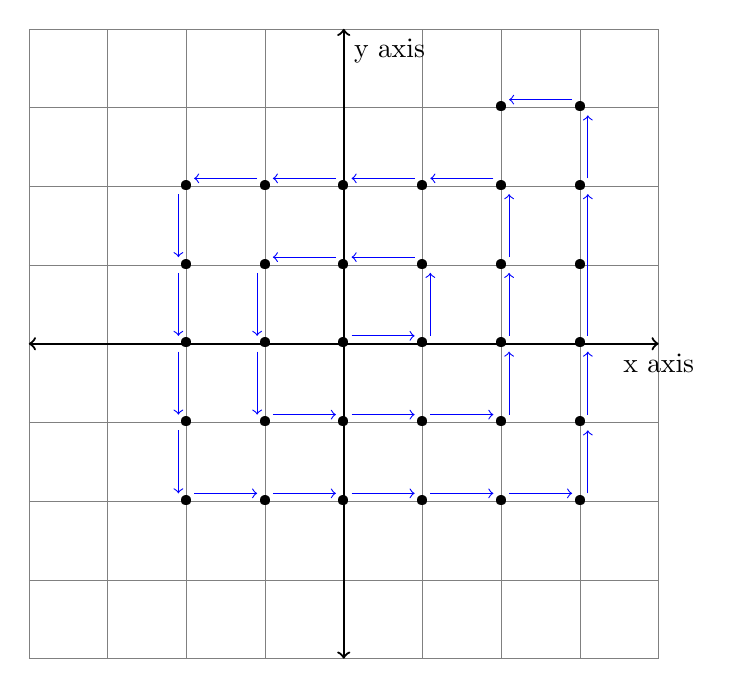
\begin{tikzpicture}
\draw[step=1cm,gray,very thin] (-4,-4) grid (4,4);
\draw[thick, ->] (0,0) -- (4,0) node[anchor=north] {x axis};
\draw[thick, ->] (0,0) -- (-4,0);
\draw[thick, ->] (0,0) -- (0,4) node[anchor=north west] {y axis};
\draw[thick, ->] (0,0) -- (0,-4);
\foreach \Point in {(0,0), (1,0), (1,1), (0,1), (-1,1), (-1,0), (-1,-1), (0,-1), (1,-1), (2,-1), (2,0), (2,1), (2,2), (1,2), (0,2), (-1,2),(-2,2), (-2,1), (-2,0), (-2, -1), (-2,-2), (-1,-2), (0,-2), (1,-2), (2,-2), (3,-2), (3,-1), (3,0), (3,1), (3,2), (3,3), (2,3)}{
    \node at \Point {\textbullet};}
\draw[draw=blue, ->] (0.1,0.1) -- (0.9, 0.1);
\draw[draw=blue, ->] (1.1,0.1) -- (1.1, 0.9);
\draw[draw=blue, ->] (0.9,1.1) -- (0.1, 1.1);
\draw[draw=blue, ->] (-0.1,1.1) -- (-0.9, 1.1);
\draw[draw=blue, ->] (-1.1,0.9) -- (-1.1, 0.1);
\draw[draw=blue, ->] (-1.1,-0.1) -- (-1.1, -0.9);
\draw[draw=blue, ->] (-0.9,-0.9) -- (-0.1, -0.9);
\draw[draw=blue, ->] (0.1,-0.9) -- (0.9, -0.9);
\draw[draw=blue, ->] (1.1,-0.9) -- (1.9, -0.9);
\draw[draw=blue, ->] (2.1,-0.9) -- (2.1, -0.1);
\draw[draw=blue, ->] (2.1,0.1) -- (2.1, 0.9);
\draw[draw=blue, ->] (2.1,1.1) -- (2.1, 1.9);
\draw[draw=blue, ->] (1.9,2.1) -- (1.1, 2.1);
\draw[draw=blue, ->] (0.9,2.1) -- (0.1, 2.1);
\draw[draw=blue, ->] (-0.1,2.1) -- (-0.9, 2.1);
\draw[draw=blue, ->] (-1.1,2.1) -- (-1.9, 2.1);
\draw[draw=blue, ->] (-2.1,1.9) -- (-2.1, 1.1);
\draw[draw=blue, ->] (-2.1,0.9) -- (-2.1, 0.1);
\draw[draw=blue, ->] (-2.1,-0.1) -- (-2.1, -0.9);
\draw[draw=blue, ->] (-2.1,-1.1) -- (-2.1, -1.9);
\draw[draw=blue, ->] (-1.9,-1.9) -- (-1.1, -1.9);
\draw[draw=blue, ->] (-0.9,-1.9) -- (-0.1, -1.9);
\draw[draw=blue, ->] (0.1,-1.9) -- (0.9, -1.9);
\draw[draw=blue, ->] (1.1,-1.9) -- (1.9, -1.9);
\draw[draw=blue, ->] (2.1,-1.9) -- (2.9, -1.9);
\draw[draw=blue, ->] (3.1,-1.9) -- (3.1, -1.1);
\draw[draw=blue, ->] (3.1,-0.9) -- (3.1, -0.1);
\draw[draw=blue, ->] (3.1,0.1) -- (3.1, 1.9);
\draw[draw=blue, ->] (3.1,2.1) -- (3.1, 2.9);
\draw[draw=blue, ->] (2.9,3.1) -- (2.1, 3.1);
\end{tikzpicture}

\end{itemize}
\end{scriptsize}
\end{frame}



\begin{frame}[fragile]
\frametitle{Countable and Uncountable}
%\framesubtitle{HOMEWORK}
\begin{scriptsize}
\begin{itemize}
\item<1-> HOMEWORK: 12, 14

\item<1-> QUIZ: 17 (due in a week)

\end{itemize}
\end{scriptsize}
\end{frame}




\section{Types of Proofs}

\begin{frame}[fragile]
\frametitle{Types of Proofs}
%\framesubtitle{HOMEWORK}
\begin{scriptsize}
\begin{itemize}
\item<1-> A proof is an argument that establishes that a hypothesis is true

\item<1-> It uses assumptions to reach a conclusion

\item<1-> Developing a proof is challenging!

\item<2-> Some fundamental proof techniques that can help guide the process: formal logic proofs, mathematical induction proofs, pigeonhole principle proofs, proofs by contradiction, and diagonalization proofs

\item<3-> Precisely state the assumptions and state the conclusion (the statement you want to prove)

\item<3-> Failing to do so is tantamount to writing a function without knowing its inputs and its purpose
\end{itemize}
\end{scriptsize}
\end{frame}

\begin{frame}[fragile]
\frametitle{Types of Proofs}
\framesubtitle{Formal Logic Proofs}
\begin{scriptsize}
\begin{itemize}
\item<1-> We are mostly interested in proving conjunctions, disjunctions, implications and equivalences

\item<2-> A conjunction that is true means that all input statements are true

\item<2->
\begin{center}
\[
\begin{tabular}{|c|c|c|}
  \hline
  % after \\: \hline or \cline{col1-col2} \cline{col3-col4} ...
  A & B & A $\wedge$ B \\ \hline
  False & False & False \\ \hline
  False &  True & False \\ \hline
   True & False & False \\ \hline
   True &  True &  True \\ \hline
\end{tabular}
\]
\end{center}

\item<2-> This means that if we wish to prove a conjunction true we must demonstrate that the input statements are true

\item<3-> Prove:
\begin{alltt}
     28 + 2 + 1 = 31 \(\wedge\) 2 * 3 + 4 = 10
\end{alltt}

\item<4->
\begin{alltt}
         30 + 1 = 31 \(\wedge\)     6 + 4 = 10
             31 = 31 \(\wedge\)        10 = 10
\end{alltt}
\end{itemize}
\end{scriptsize}
\end{frame}

\begin{frame}[fragile]
\frametitle{Types of Proofs}
\framesubtitle{Formal Logic Proofs}
\begin{scriptsize}
\begin{itemize}
\item<1-> A disjunction that is true means that any of its input statements are true

\item<2-> The following is the truth table for \texttt{$\vee$} with two input statements:
\begin{center}
\[
\begin{tabular}{|c|c|c|}
  \hline
  % after \\: \hline or \cline{col1-col2} \cline{col3-col4} ...
  A & B & A $\vee$ B \\ \hline
  False & False & False \\ \hline
  False &  True &  True \\ \hline
   True & False &  True \\ \hline
   True &  True &  True \\ \hline
\end{tabular}
\]
\end{center}

\item<2-> If we wish to prove a disjunction true we must demonstrate that at least one of its input statements is true

\item<3->
\begin{alltt}
     7 + 1 + 3 > 20  \(\vee\)  -2 * 2 + 4 \(\geq\) 0  \(\vee\)  x \(\geq\) x + x + x
\end{alltt}
\item<4->
\begin{alltt}
     7 + 1 + 3 > 20  \(\vee\)  -2 * 2 + 4 \(\geq\) 0  \(\vee\)  x \(\geq\) x + x + x
         8 + 3 > 20  \(\vee\)     -4 + 4  \(\geq\) 0  \(\vee\)  x \(\geq\) x + 2x
            11 > 20  \(\vee\)          0  \(\geq\) 0  \(\vee\)  x \(\geq\) 3x
\end{alltt}
Clearly, \texttt{0 \(\geq\) 0}. Therefore, we may conclude that the disjunction holds.
\end{itemize}
\end{scriptsize}
\end{frame}

\begin{frame}[fragile]
\frametitle{Types of Proofs}
\framesubtitle{Formal Logic Proofs}
\begin{scriptsize}
\begin{itemize}
\item<1-> We must know how to prove an implication: \texttt{A $\Rightarrow$ B}

\item<1-> \texttt{A} is the antecedent and \texttt{B} is the consequent

\item<1-> It states that if \texttt{A} is true then \texttt{B} is also true:
\begin{center}
\[
\begin{tabular}{|c|c|c|}
  \hline
  % after \\: \hline or \cline{col1-col2} \cline{col3-col4} ...
  A & B & A $\Rightarrow$ B \\ \hline
  False & False &  True \\ \hline
  False &  True &  True \\ \hline
   True & False &  False \\ \hline
   True &  True &  True \\ \hline
\end{tabular}
\]
\end{center}

\item<2-> When the antecedent is true then the consequent is also true.

\item<2-> Assume the antecedent is true and demonstrate that the consequent is true

\item<3->
\begin{alltt}
     3x - 9 \(\geq\) 0 \(\Rightarrow\) x \(\geq\) 3
\end{alltt}

\item<4-> Assume that \texttt{3x - 9 \(\geq\) 0} is true

\item<4-> We must show that \texttt{x \(\geq\) 3} is true

\item<5->
\begin{alltt}
     3x - 9 \(\geq\) 0 \(\Rightarrow\) x \(\geq\) 3
         3x \(\geq\) 9 \(\Rightarrow\) x \(\geq\) 3
          x \(\geq\) 3 \(\Rightarrow\) x \(\geq\) 3
\end{alltt}

\end{itemize}
\end{scriptsize}
\end{frame}

\begin{frame}[fragile]
\frametitle{Types of Proofs}
\framesubtitle{Formal Logic Proofs}
\begin{scriptsize}
\begin{itemize}
\item<1-> Logical equivalence: \texttt{A $\Leftrightarrow$ B}:
\begin{alltt}
     A \(\Rightarrow\) B \(\wedge\) B \(\Rightarrow\) A
\end{alltt}

\item<2->
\begin{center}
\[
\begin{tabular}{|c|c|c|}
  \hline
  % after \\: \hline or \cline{col1-col2} \cline{col3-col4} ...
  A & B & A $\Leftrightarrow$ B \\ \hline
  False & False &  True \\ \hline
  False &  True &  False \\ \hline
   True & False &  False \\ \hline
   True &  True &  True \\ \hline
\end{tabular}
\]
\end{center}

\item<2-> Holds when both input statements have the same value

\item<2-> Proving logical equivalence requires proving two implications

\item<3->
\begin{alltt}
  x is a square \(\Leftrightarrow\) \(\sqrt{x}\)\(\in\mathbb{N}\)
\end{alltt}

\item<4-> We must prove that:
\begin{enumerate}
  \item \texttt{x is a square \(\Rightarrow\) \(\sqrt{x}\) \(\in \mathbb{N}\)}
  \item \texttt{\(\sqrt{x} \in \mathbb{N} \Rightarrow\) x is a square}
\end{enumerate}

\item<5-> Assume \texttt{x is a square}:
\begin{alltt}
     x is a square \(\Rightarrow\) x = k * k, k \(\in\) \(\mathbb{N}\)
                   \(\Rightarrow\) \(\sqrt{x}\) = k
                   \(\Rightarrow\) \(\sqrt{x}\in\mathbb{N}\)
\end{alltt}

\item<6-> Assume \texttt{\(\sqrt{x} \in \mathbb{N}\)}:
\begin{alltt}
     \(\sqrt{x} \in \mathbb{N}\) \(\Rightarrow\) x = k * k
         \hspace{0.08cm}     \(\Rightarrow\) x = k\(\sp{2}\)
\end{alltt}

\end{itemize}
\end{scriptsize}
\end{frame}

\begin{frame}[fragile]
\frametitle{Types of Proofs}
\framesubtitle{Formal Logic Proofs}
\begin{scriptsize}
\begin{itemize}
\item<1-> Universal quantification states that for all members of a set some predicate holds

\item<2->
\begin{alltt}
     M4 = \{n | n \(\in \mathbb{N} \wedge\) n is a multiple of 4\}
\end{alltt}

\item<3-> We can make statements about all the members of \texttt{M4}:
\begin{alltt}
     \(\forall\) n \(\in\) M4 n = 2k, where k \(\in \mathbb{N}\)
\end{alltt}


\item<4-> To prove a statement using universal quantification we must argue that the statement is true for an arbitrary member of the set:

\item<5->
\begin{alltt}
     Let \texttt{x} be an arbitrary member of \texttt{M4}.

     \texttt{x} \(\in\) \texttt{M4} \(\Rightarrow\) x = 4\texttt{h}\\
            \(\Rightarrow\) x = 2*2*\texttt{h}\\
            \(\Rightarrow\) x = 2\texttt{k}, where \texttt{k} = 2\texttt{h} \(\qed\)
\end{alltt}

\end{itemize}
\end{scriptsize}
\end{frame}

\begin{frame}[fragile]
\frametitle{Types of Proofs}
\framesubtitle{Formal Logic Proofs}
\begin{scriptsize}
\begin{itemize}
\item<1-> Existential quantification states that there exists a member of the set for which a predicate holds

\item<2->
\begin{alltt}
     \(\exists\) n \(\in\) M4 n is a multiple of 5
\end{alltt}

\item<3-> To prove a statement using existential quantification we must demonstrate that a specific member of the set satisfies the predicate

\item<4->
\begin{alltt}
     Let x = 20.

     x = 20 \(\Rightarrow\) x = 4 * 5
            \(\Rightarrow\) x \(\in\) M4 \(\wedge\) x is a multiple of 5 \(\qed\)
\end{alltt}

\end{itemize}
\end{scriptsize}
\end{frame}

\begin{frame}[fragile]
\frametitle{Types of Proofs}
\framesubtitle{Formal Logic Proofs}
\begin{scriptsize}
\begin{itemize}
\item<1-> HOMEWORK: 1--10

\end{itemize}
\end{scriptsize}
\end{frame}

\begin{frame}[fragile]
\frametitle{Types of Proofs}
\framesubtitle{Mathematical Induction}
\begin{scriptsize}
\begin{itemize}
\item<1-> We define the set of natural numbers, \texttt{$\mathbb{N}$}, as follows:
\begin{alltt}
     A natural number is either:
       1. 0
       2. n + 1, where n \(\in\) \(\mathbb{N}\)
\end{alltt}

\item<2-> We say that 0 is a base instance of $\mathbb{N}$: a value known to be in the set

\item<2-> A set may have more than one base value

\item<3-> Values that are not base values (let us call them inductive values) must be constructed from other elements in the set

\item<4-> 5 is a natural number:
\begin{alltt}
     0 \(\in \mathbb{N}\) \(\Rightarrow\) 1 \(\in \mathbb{N}\)
     \hspace{0.2cm}      \(\Rightarrow\) 2 \(\in \mathbb{N}\)
     \hspace{0.2cm}      \(\Rightarrow\) 3 \(\in \mathbb{N}\)
     \hspace{0.2cm}      \(\Rightarrow\) 4 \(\in \mathbb{N}\)
     \hspace{0.2cm}      \(\Rightarrow\) 5 \(\in \mathbb{N}\)
\end{alltt}
\end{itemize}
\end{scriptsize}
\end{frame}

\begin{frame}[fragile]
\frametitle{Types of Proofs}
\framesubtitle{Mathematical Induction}
\begin{scriptsize}
\begin{itemize}
\item<1-> What is required to prove that a predicate holds $\forall \ \mathbb{N}$?

\item<2-> The definition suggests that such a proof must have two parts

\item<2-> The first part establishes that the predicate holds for the base value (i.e., 0)

\item<3-> Second part establishes the predicate holds for the inductive instances

\item<4-> The second part, however, requires special care:
\begin{alltt}
     Prove P(1) holds
     Prove P(2) holds
     Prove P(3) holds
          \(\vdots\)
\end{alltt}

\item<5-> We must rely on the implication suggested by the data definition:
\begin{alltt}
     n \(\in\) \(\mathbb{N}\) \(\Rightarrow\) n + 1 \(\in\) \(\mathbb{N}\)
\end{alltt}

\item<6-> Suggests that we must show: \texttt{P(n) holds \(\Rightarrow\) P(n+1) holds}


\item<7-> The good news is that we know how to prove an implication

\item<7-> \texttt{P(n)} is called the inductive hypothesis.

\item<8-> This is the principal of \emph{mathematical induction}:
\begin{enumerate}
  \item Prove the base case
  \item The inductive step
    \begin{enumerate}
      \item State, \texttt{P(k)}, the inductive hypothesis
      \item State, \texttt{P(k+1)}, what must be proven
      \item Assume \texttt{P(k)} is true and prove \texttt{P(k+1)}
    \end{enumerate}
\end{enumerate}

\item<8-> The inductive hypothesis is valid for all values in \texttt{[0..k]}
\end{itemize}
\end{scriptsize}
\end{frame}

\begin{frame}[fragile]
\frametitle{Types of Proofs}
\framesubtitle{Mathematical Induction}
\begin{scriptsize}
\begin{itemize}
\item<1->
\begin{alltt}
     #lang fsm

     ;; natnum \arrow natnum
     ;; Purpose: Compute the square of the given natnum
     (define (square n)
       (if (= n 0)
           0
           (+ (sub1 (* 2 n)) (square (sub1 n)))))

     ;; Tests
     (check-equal? (square 0)   0)
     (check-equal? (square 5)   25)
     (check-equal? (square 100) 10000)
\end{alltt}

\item<2-> Can you prove that the function is correct?


\end{itemize}
\end{scriptsize}
\end{frame}

\begin{frame}[fragile]
\frametitle{Types of Proofs}
\framesubtitle{Mathematical Induction}
\begin{scriptsize}
\begin{itemize}
\item<1->
\begin{alltt}
     ;; natnum \arrow natnum
     ;; Purpose: Compute the square of the given natnum
     (define (square n)
       (if (= n 0)
           0
           (+ (sub1 (* 2 n)) (square (sub1 n)))))
\end{alltt}

\item<2->
\begin{theorem}
(square n) returns n$^{2}$
\end{theorem}
\begin{proof}
\mbox{}\\
\noindent \underline{Base Case}: n = 0

If n = 0 then \texttt{(square n)} = \texttt{(square 0)} returns 0 = 0$^2$ = n$^2$

\noindent \underline{Inductive Step}:\\
Assume: \texttt{(square k)} returns k$^2$, for n = k $\geq$ 0\\

\noindent Show that: \texttt{(square (add1 k))} returns \texttt{(add1 k)}$^2$\\

\noindent k $\geq$ 0 $\Rightarrow$ \texttt{(add1 k)} $>$ 0\\
\mbox{} \hspace{0.75cm} $\Rightarrow$ \texttt{(square k+1)} returns \texttt{(+ (sub1 (* 2 (add1 k))) (square k))}\\
\mbox{} \hspace{0.75cm} $\Rightarrow$ \texttt{(square k+1)} returns \texttt{(+ (sub1 (+ (* 2 k)  2)) k$^2$)}\\
\mbox{} \hspace{0.75cm} $\Rightarrow$ \texttt{(square k+1)} returns \texttt{(+ (+ (* 2 k)  1)) k$^2$)}\\
\mbox{} \hspace{0.75cm} $\Rightarrow$ \texttt{(square k+1)} returns \texttt{(add1 k)$^2$} $\qed$
\end{proof}
\end{itemize}
\end{scriptsize}
\end{frame}

\begin{frame}[fragile]
\frametitle{Types of Proofs}
\framesubtitle{Mathematical Induction}
\begin{scriptsize}
\begin{itemize}
\item<1-> HOMEWORK: 11--13
\end{itemize}
\end{scriptsize}
\end{frame}

\begin{frame}[fragile]
\frametitle{Types of Proofs}
\framesubtitle{Pigeonhole Principle}
\begin{scriptsize}
\begin{itemize}
\item<1-> Imagine that in a colony of pigeons you have 50 pigeons and 45 pigeonholes

\item<1-> It is impossible to place each pigeon in its own pigeonhole

\item<2-> A one-to-one function from the set of pigeons to the set of pigeonholes does not exists

\item<2-> This observation leads to \emph{the pigeonhole principle}.
\end{itemize}
\end{scriptsize}
\end{frame}

\begin{frame}[fragile]
\frametitle{Types of Proofs}
\framesubtitle{Pigeonhole Principle}
\begin{scriptsize}
\begin{itemize}

\begin{theorem}
\texttt{A} and \texttt{B} are finite sets $\wedge$ \texttt{|A|} $>$ \texttt{|B|} $\Rightarrow$ $\nexists$ a one-to-one function from \texttt{A} to \texttt{B}.
\end{theorem}

\item<1-> We shall prove the theorem by induction on \texttt{n} = \texttt{|B|}.

\item<2->
%\begin{proof}
%\mbox{}\\
\underline{Base Case}: n = 0 (i.e., \texttt{B} = $\emptyset$)\\
\noindent There is no function from \texttt{A} to \texttt{B}, because nothing can be mapped to elements of \texttt{B}. No function from \texttt{A} to \texttt{B} $\Rightarrow$ no one-to-one function from \texttt{A} to \texttt{B}.

\item<3->
\noindent \underline{Inductive Step}\\
Assume: \texttt{f:A $\rightarrow$ B} is not a one-to-one function such that \texttt{|A|}$>$\texttt{|B|}, \texttt{|B|}$\leq$\texttt{n}, and \texttt{n} $\geq$ 0.\\
We must show: \texttt{f: A $\rightarrow$ B} is not a one-to-one function such that \texttt{|A|} $>$ \texttt{|B|} $=$ \texttt{n+1}.\\

\item<4-> Observe that \texttt{A} has at least 2 elements because \texttt{n+1} $>$ 0. Pick two distinct arbitrary elements, \texttt{a} and \texttt{b}, from \texttt{A}. If \texttt{f(a)} $=$ \texttt{f(b)} then \texttt{f} is not one-to-one (because two distinct elements of \texttt{A} map to the same element in \texttt{B}).
\item<5-> If \texttt{f(a)} $\neq$ \texttt{f(b)} suppose that \texttt{a} is the only element mapped to \texttt{f(a)}. Consider the sets \texttt{A\textquotesingle{} = A - \{a\}} and \texttt{B\textquotesingle{} = B - \{f(a)\}} and a function \texttt{f\textquotesingle{}} such that $\forall$ \texttt{x} $\in$ \texttt{A\textquotesingle{}} \texttt{f\textquotesingle{}(x)} = \texttt{f(x)}. The inductive hypothesis applies because \texttt{|B\textquotesingle{}|} = \texttt{n} and \texttt{|A\textquotesingle{}|} $>$ \texttt{|B\textquotesingle{}|}. This means that there are two distinct elements in \texttt{A\textquotesingle{}} that are mapped by \texttt{f\textquotesingle{}} to the same element of \texttt{B\textquotesingle{}}. Given that \texttt{f} agrees with \texttt{f\textquotesingle{}} on all elements, it follows that \texttt{f} is not one-to-one.
%\end{proof}

\end{itemize}
\end{scriptsize}
\end{frame}

\begin{frame}[fragile]
\frametitle{Types of Proofs}
\framesubtitle{Pigeonhole Principle}
\begin{scriptsize}
\begin{itemize}
\item<1-> \begin{theorem}
Let \texttt{G} be a graph with \texttt{n} nodes. Any path with \texttt{n} edges has a repeated node.
\end{theorem}

\item<2->
\begin{proof}
Every edge connects two nodes (not necessarily distinct nodes). This means that \texttt{n} edges connect \texttt{n+1} nodes. By the pigeonhole principle there is no one-to-one function from the nodes in the path (the pigeons) to the nodes in the graph (the pigeonholes). Therefore, we may conclude that there is at least one node repeated in the path.
\end{proof}
\end{itemize}
\end{scriptsize}
\end{frame}

\begin{frame}[fragile]
\frametitle{Types of Proofs}
\framesubtitle{Pigeonhole Principle}
\begin{scriptsize}
\begin{itemize}
\item<1-> HOMEWORK: 14--16
\end{itemize}
\end{scriptsize}
\end{frame}

\begin{frame}[fragile]
\frametitle{Types of Proofs}
\framesubtitle{Proofs by Contradiction}
\begin{scriptsize}
\begin{itemize}
\item<1-> A proof by contradiction proves that a statement holds by showing that assuming that the statement is false is absurd

\item<1-> Also known as \emph{reductio ad absurdum}

\item<2-> It is based on the observation that a statement cannot be both true and false

\item<3-> A proof by contradiction establishes that the negation of a statement leads to such a contradiction

\item<3-> Assuming \texttt{S} is false leads to concluding that a statement \texttt{A}, that we know to be false, is true

\item<3-> This means that our assumption must be wrong and, therefore, \texttt{S} must be true.
\end{itemize}
\end{scriptsize}
\end{frame}

\begin{frame}[fragile]
\frametitle{Types of Proofs}
\framesubtitle{Proofs by Contradiction}
\begin{scriptsize}
\begin{itemize}
\begin{theorem}
$\sqrt{2}$ is an irrational number
\end{theorem}

\item<2->
\noindent Assume $\sqrt{2}$ is a rational number

\item<3->
\noindent If $\sqrt{2}$ is rational then it can be expressed as a fraction, $\frac{a}{b}$, in lowest terms for \texttt{a,b $\in \mathbb{Z}$}

\item<4-> Observe that at least one of \texttt{a} and \texttt{b} must be odd

\item<4-> Consider:
$\frac{a}{b}$ = $\sqrt{2}$\\
$\frac{a^2}{b^2}$ = 2\\
$a^2$ = 2$b^2$\\

\item<4-> This means that \texttt{$a^2$} is even

\item<5-> Observe that this also means that \texttt{a} is even because \texttt{a * a} must be divisible by 2 (if \texttt{a} were odd then \texttt{a * a} would not be divisible by 2)

\item<6-> Given that \texttt{a} is even and $\frac{a}{b}$ is in lowest terms, \texttt{b} must be odd (otherwise, \texttt{a} and \texttt{b} have 2 as a common factor)

\item<7-> Observe that \texttt{$a^2$} is a multiple of 4:\\
\texttt{$a^2$} = \texttt{$a * a$} = \texttt{$2j * 2j$} = \texttt{$4j^2$}\\

\item<8-> This means that 2$b^2$ is a multiple of 4. We observe that \texttt{b} must be even given that if it were odd \texttt{b} could equal 3 which means 2$b^2$ is not a multiple of 4 (i.e., 2(3)$^2$ = 18 which is not a multiple of 4)

\item<9-> It is impossible, however, for \texttt{b} to be both odd and even

\item<9-> Our assumption cannot be true and we may conclude that $\sqrt{2}$ is an irrational number.
\end{itemize}
\end{scriptsize}
\end{frame}

\begin{frame}[fragile]
\frametitle{Types of Proofs}
\framesubtitle{Proofs by Contradiction}
\begin{scriptsize}
\begin{itemize}
\item<1-> HOMEWORK: 17--18
\end{itemize}
\end{scriptsize}
\end{frame}

\begin{frame}[fragile]
\frametitle{Types of Proofs}
\framesubtitle{Diagonalization Proofs}
\begin{scriptsize}
\begin{itemize}
\item<1-> A binary relation on a set \texttt{A} may be visualized as a matrix whose rows and columns are labeled with the elements of \texttt{A}

\item<1-> If \texttt{i} is related to \texttt{j} then the entry in row \texttt{i} and column \texttt{j} contains an \texttt{x}

\item<2->
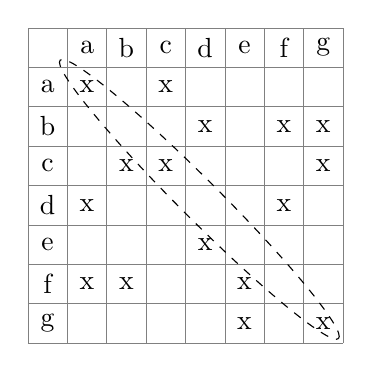
\begin{tikzpicture}[scale=0.5]
\draw[step=1cm,gray,very thin] (-4,-4) grid (4,4);
\draw (-3.5,2.5) node{a};
\draw (-3.5,1.5) node{b};
\draw (-3.5,0.5) node{c};
\draw (-3.5,-0.5) node{d};
\draw (-3.5,-1.5) node{e};
\draw (-3.5,-2.5) node{f};
\draw (-3.5,-3.5) node{g};
\draw (-2.5,3.5) node{a};
\draw (-1.5,3.5) node{b};
\draw (-0.5,3.5) node{c};
\draw (0.5,3.5) node{d};
\draw (1.5,3.5) node{e};
\draw (2.5,3.5) node{f};
\draw (3.5,3.5) node{g};
\draw (-2.5,2.5) node{x}; % a row
\draw (-0.5,2.5) node{x};
\draw (0.5,1.5) node{x}; %b row
\draw (2.5,1.5) node{x};
\draw (3.5,1.5) node{x};
\draw (-1.5,0.5) node{x}; % c row
\draw (-0.5,0.5) node{x};
\draw (3.5,0.5) node{x};
\draw (-2.5,-0.5) node{x}; %d row
\draw (2.5,-0.5) node{x};
\draw (0.5,-1.5) node{x}; % e row
\draw (1.5,-2.5) node{x}; % f row
\draw (-1.5,-2.5) node{x};
\draw (-2.5,-2.5) node{x};
\draw (3.5,-3.5) node{x}; % g row
\draw (1.5,-3.5) node{x};
\draw[rotate=-45,black,dashed] (0:5.5cm and 2cm) arc (0:360:5cm and 0.5cm);
\end{tikzpicture}

\end{itemize}
\end{scriptsize}
\end{frame}

\begin{frame}[fragile]
\frametitle{Types of Proofs}
\framesubtitle{Diagonalization Proofs}
\begin{scriptsize}
\begin{itemize}
\item<1->
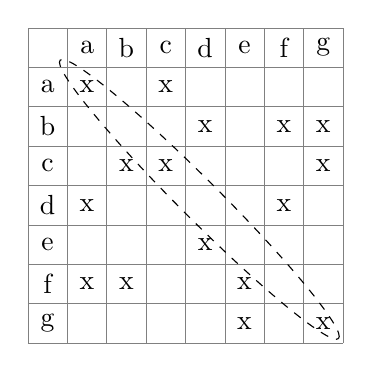
\begin{tikzpicture}[scale=0.5]
\draw[step=1cm,gray,very thin] (-4,-4) grid (4,4);
\draw (-3.5,2.5) node{a};
\draw (-3.5,1.5) node{b};
\draw (-3.5,0.5) node{c};
\draw (-3.5,-0.5) node{d};
\draw (-3.5,-1.5) node{e};
\draw (-3.5,-2.5) node{f};
\draw (-3.5,-3.5) node{g};
\draw (-2.5,3.5) node{a};
\draw (-1.5,3.5) node{b};
\draw (-0.5,3.5) node{c};
\draw (0.5,3.5) node{d};
\draw (1.5,3.5) node{e};
\draw (2.5,3.5) node{f};
\draw (3.5,3.5) node{g};
\draw (-2.5,2.5) node{x}; % a row
\draw (-0.5,2.5) node{x};
\draw (0.5,1.5) node{x}; %b row
\draw (2.5,1.5) node{x};
\draw (3.5,1.5) node{x};
\draw (-1.5,0.5) node{x}; % c row
\draw (-0.5,0.5) node{x};
\draw (3.5,0.5) node{x};
\draw (-2.5,-0.5) node{x}; %d row
\draw (2.5,-0.5) node{x};
\draw (0.5,-1.5) node{x}; % e row
\draw (1.5,-2.5) node{x}; % f row
\draw (-1.5,-2.5) node{x};
\draw (-2.5,-2.5) node{x};
\draw (3.5,-3.5) node{x}; % g row
\draw (1.5,-3.5) node{x};
\draw[rotate=-45,black,dashed] (0:5.5cm and 2cm) arc (0:360:5cm and 0.5cm);
\end{tikzpicture}

\item<1-> The main diagonal of the visualization of binary relation defines two sets: those elements that are related to themselves and those elements that are not related to themselves

\item<2-> Formally:
\begin{alltt}
     D = \{a | (a, a) \(\in\) R\}    \^{D} = \{a | (a, a) \(\notin\) R\}
\end{alltt}

\item<3-> The \emph{diagonalization principle} states that \texttt{\^{D}} is not equal to any row in the visualization: \texttt{\^{D}} \texttt{$\neq$} \texttt{R$_{\texttt{a}}$}

\item<4-> The diagonalization principle is used as part of a proof by contradiction

\item<4-> A statement is assumed to be true and diagonalization is used to develop a contradiction

\end{itemize}
\end{scriptsize}
\end{frame}

\begin{frame}[fragile]
\frametitle{Types of Proofs}
\framesubtitle{Diagonalization Proofs}
\begin{scriptsize}
\begin{itemize}
\item<1-> Prove that the real numbers in \texttt{(0..1)} are uncountable

\item<1-> We shall use a well-known fact for computer scientists: every real number in \texttt{(0..1)} may be written as a binary number of infinite length

\end{itemize}
\end{scriptsize}
\end{frame}

\begin{frame}[fragile]
\frametitle{Types of Proofs}
\framesubtitle{Diagonalization Proofs}
\begin{scriptsize}
\begin{itemize}
\begin{theorem}
The set of real numbers in \texttt{(0..1)} is uncountable.
\end{theorem}

\item<2->
\begin{proof}
\mbox{}\\
Assume the set of real numbers in \texttt{(0..1)} is countable.\\

This means there exists a program to print these numbers that eventually prints any arbitrary binary digit of any real number in \texttt{(0..1)}. The printing of these real numbers looks as follows:
\begin{alltt}
     1. .0 0 0 1 0 1 1 \dotss
     2. .1 1 0 1 0 0 0 \dotss
     3. .0 1 0 0 0 0 0 \dotss
     4. .0 1 1 0 0 0 1 \dotss
     5. .0 0 0 0 1 1 0 \dotss
     6. .1 1 1 1 1 1 1 \dotss
     7. .1 1 0 0 0 0 0 \dotss
          \vdotss
\end{alltt}
Observe that the binary digits form a matrix. Consider the real number represented by \texttt{\^{D}}. \texttt{\^{D}} cannot ever equal an arbitrary row \texttt{i} in the matrix of printed numbers because their \texttt{i$^{\texttt{th}}$} bits differ. This means that the real number represented by \texttt{\^{D}} is never be printed. This contradicts the assumption made that the set of real numbers in \texttt{(0..1)} are countable and, therefore, the set of real numbers in \texttt{(0..1)} is uncountable. $\qed$
\end{proof}
\end{itemize}
\end{scriptsize}
\end{frame}

\begin{frame}[fragile]
\frametitle{Types of Proofs}
\framesubtitle{Diagonalization Proofs}
\begin{scriptsize}
\begin{itemize}
\item<1-> Recall that in the previous chapter we tabled the discussion on whether or not \texttt{$\mathbb{R}$}, and, \texttt{$\mathbb{Z}$} are equinumerous
    
\item<2-> Observe that the previous proof means that there is no bijection between \texttt{$\mathbb{N}$} and \texttt{$\mathbb{R}$}
     
\item<2->  That is, \texttt{$\mathbb{N}$} and \texttt{$\mathbb{R}$} are not equinumerous
    
\item<3-> We know from the previous chapter that \texttt{$\mathbb{N}$} and \texttt{$\mathbb{Z}$} are equinumerous
    
\item<4-> Therefore, their does not exist a bijection between \texttt{$\mathbb{R}$} and \texttt{$\mathbb{Z}$}
    
\item<4-> These sets are not equinumerous

\end{itemize}
\end{scriptsize}
\end{frame}

\begin{frame}[fragile]
\frametitle{Types of Proofs}
\framesubtitle{Diagonalization Proofs}
\begin{scriptsize}
\begin{itemize}
\item<1-> HOMEWORK: 19--20

\item<1-> QUIZ: 21 (due in 1 week)
\end{itemize}
\end{scriptsize}
\end{frame}

\end{document} 